\section{3 einfache Sortieralgorithmen}

\begin{center}
	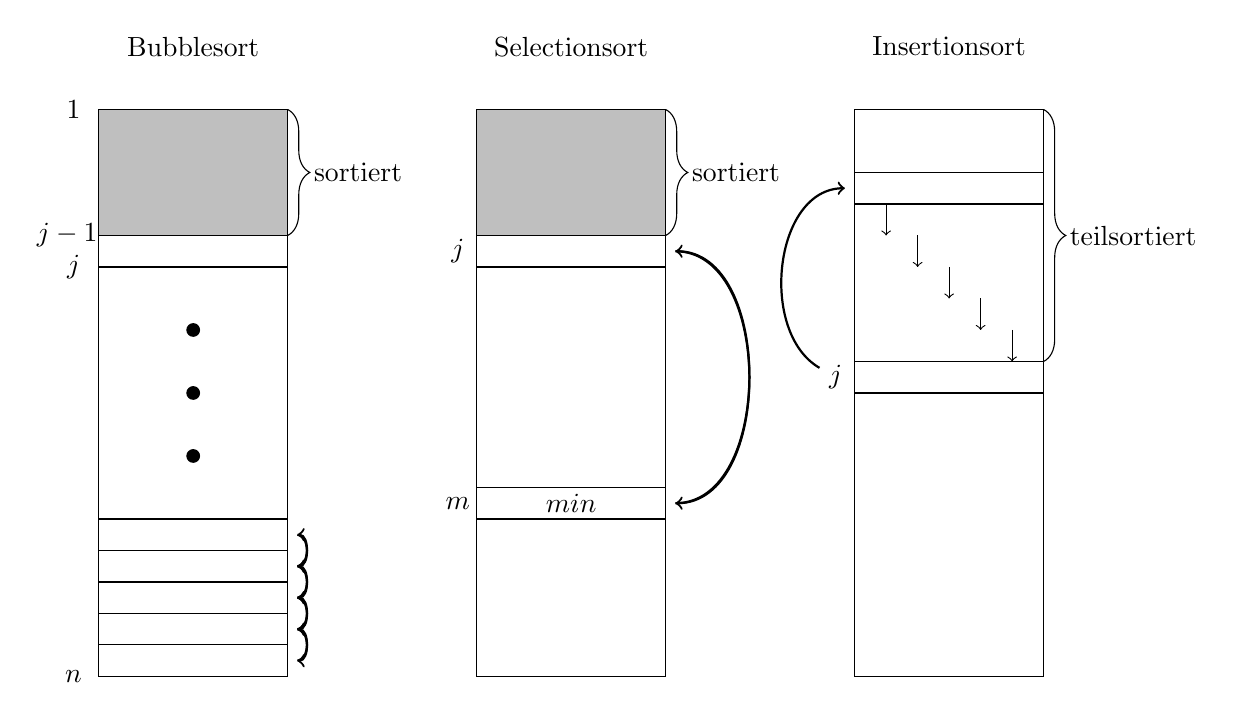
\begin{tikzpicture}[scale=0.8]
	\node at (1.5,1) (bubble) {Bubblesort};
	\draw (0,0) rectangle (3,-9);
	\draw[fill=lightgray] (0,0) rectangle (3,-2);
	\draw[decorate,decoration={brace,amplitude=8pt}] (3,0) -- (3,-2) node[midway, right, xshift=6pt]{sortiert};
	\draw (0,-2.5) -- (3,-2.5);
	\draw[fill=black] (1.5,-3.5) circle (0.1);
	\draw[fill=black] (1.5,-4.5) circle (0.1);
	\draw[fill=black] (1.5,-5.5) circle (0.1);
	\draw (0,-6.5) -- (3,-6.5);
	\draw (0,-7) -- (3,-7);
	\draw (0,-7.5) -- (3,-7.5);
	\draw (0,-8) -- (3,-8);
	\draw (0,-8.5) -- (3,-8.5);
	
	\node at (-0.4,0) (1) {1};
	\node at (-0.5,-2) (j-1) {$j-1$};
	\node at (-0.4,-2.5) (j) {$j$};
	\node at (-0.4,-9) (n) {$n$};
	
	\node at (3,-6.75) (a) {};
	\node at (3,-7.25) (b) {};
	\node at (3,-7.75) (c) {};
	\node at (3,-8.25) (d) {};
	\node at (3,-8.75) (e) {};
	\draw[->, thick] (a) to [out=0, in=0] (b);
	\draw[->, thick] (b) to [out=0, in=0] (c);
	\draw[->, thick] (c) to [out=0, in=0] (d);
	\draw[->, thick] (d) to [out=0, in=0] (e);
	\draw[->, thick] (e) to [out=0, in=0] (d);
	\draw[->, thick] (d) to [out=0, in=0] (c);
	\draw[->, thick] (c) to [out=0, in=0] (b);
	\draw[->, thick] (b) to [out=0, in=0] (a);
	
	\node at (7.5,1) (selection) {Selectionsort};
	\draw (6,0) rectangle (9,-9);
	\draw[fill=lightgray] (6,0) rectangle (9,-2);
	\draw[decorate,decoration={brace,amplitude=8pt}] (9,0) -- (9,-2) node[midway, right, xshift=6pt]{sortiert};
	\draw (6,-2.5) -- (9,-2.5);
	\node at (5.7,-2.25) (j) {$j$};
	\draw (6,-6.5) -- (9,-6.5);
	\node at (5.7,-6.25) (m) {$m$};
	\draw (6,-6) -- (9,-6);
	\node at (7.5,-6.25) (min) {$min$};
	
	\node at (9,-2.25) (g) {};
	\node at (9,-6.25) (h) {};
	\draw[->,thick] (h) to [out=0, in=0] (g);
	\draw[->,thick] (g) to [out=0, in=0] (h);
	
	\node at (13.5,1) (insert) {Insertionsort};
	\draw (12,0) rectangle (15,-9);
	\draw[decorate,decoration={brace,amplitude=8pt}] (15,0) -- (15,-4) node[midway, right, xshift=6pt]{teilsortiert};
	\draw (12,-4.5) -- (15,-4.5);
	\node at (11.7,-4.25) (j) {$j$};
	\draw (12,-4) -- (15,-4);
	\draw (12,-1) -- (15,-1);
	\draw (12,-1.5) -- (15,-1.5);
	\node at (12,-1.25) (k) {};
	\draw[->,thick] (j) to [out=150, in=180] (k);
	
	\draw[->] (12.5,-1.5) -- (12.5,-2);
	\draw[->] (13,-2) -- (13,-2.5);
	\draw[->] (13.5,-2.5) -- (13.5,-3);
	\draw[->] (14,-3) -- (14,-3.5);
	\draw[->] (14.5,-3.5) -- (14.5,-4);
	\end{tikzpicture}
\end{center}

\begin{tabular}{p{0.2\textwidth}|p{0.35\textwidth}|p{0.35\textwidth}}
	\cellcolor{lightgray}\textbf{Sortierverfahren} & \cellcolor{lightgray}\textbf{Anzahl Vergleiche} & \cellcolor{lightgray}\textbf{Anzahl Kopier-/Tauschoperationen} \\
	\hline
	\textbf{Bubblesort} & $\sum\limits_{j=1}^{n-1}(n-j) = \sum\limits_{j=1}^{n-1}\frac{n(n-1)}{2} = \mathcal{O}(n^2) = \Omega(n)$ & $\le\frac{1}{2}n(n-1)=\mathcal{O}(n^2)$ Tauschoperationen \\
	\hline
	\textbf{Selectionsort} & $\sum\limits_{j=1}^{n-1}\frac{n(n-1)}{2}=\Theta(n^2)$ & $\le n-1=\mathcal{O}(n)$ Tauschoperationen \\
	\hline
	\textbf{Insertionsort} & $\sum\limits_{j=1}^{n-1} j=\frac{n(n-1)}{2}=\mathcal{O}(n^2)$ & $\le\sum\limits_{j=1}^{n-1} j=\frac{n(n-1)}{2}=\mathcal{O}(n^2)$ \\
	mit binärer Suche im teilsortierten Teil & $\sum\limits_{j=1}^{n-1}\log_2 j=\mathcal{O}(n\log_2 n)$ & hier bleibt alles gleich \\
\end{tabular}

Allgemein kann man also sagen:
\begin{itemize}
	\item best case: 0 Bewegungen/Kopier- und Tauschvorgänge, $\Omega(n)$ Vergleiche
	\item worst case: $\mathcal{O}(n^2)$ Vergleiche und Kopier-/Tauschoperationen
\end{itemize}

\begin{tabularx}{\textwidth}{p{0.2\textwidth}|p{0.35\textwidth}|X}
	\cellcolor{lightgray} & \cellcolor{lightgray}\textbf{Vergleiche} & \cellcolor{lightgray}\textbf{Tauschoperationen} \\
	\hline
	\textbf{Bubblesort}, \textcolor{red}{stabil} & $\mathcal{O}(n^2)$ & $\mathcal{O}(n^2)$ \\
	\hline
	\textbf{Selectionsort}, \textcolor{red}{nicht stabil} & $\mathcal{O}(n^2)$ & $\mathcal{O}(n)$ \\
	\hline
	\textbf{Insertionsort}, \textcolor{red}{stabil} & ohne binäre Suche: $\mathcal{O}(n^2)$, mit binärer Suche: $\mathcal{O}(n\log_2 n)$ & $\mathcal{O}(n^2)$
\end{tabularx}
$\Rightarrow T(n)=\mathcal{O}(n^2)$ für alle 3 einfachen Sortierverfahren

\begin{proposition}
	Sortierverfahren, die auf dem Schlüsselvergleich ($<$) von jeweils 2 Elementen (und einer eventuell notwendigen Tauschoperation) beruhen, benötigen im worst case mindestens $\Omega(n\log_2 n)$ Vergleiche.
\end{proposition}
\begin{proof}
	binärer Entscheidungsbaum der Höhe $h$ zum Sortieren von $n$ Elementen, da jeder Schlüsselwertvergleich eine binäre Entscheidung liefert. Es gibt $n!$ Permutationen der $n$ verschiedenen Schlüsselwerte, also $n!$ verschiedene Sortierfolgen, das heißt $n!$ Entscheidungspfade. $\Rightarrow$ binärer Entscheidungsbaum benötigt mindestens $n!$ Blätter, um alle Anfangszustände in den einen Sortierten zu überführen. Ein Binärbaum der Höhe $h$ hat $\le 2^h$ Blätter. Also muss gelten:
	\begin{align}
		n! &\le 2^h \notag \\
		h &\ge \log_2(n!) \notag \\
		\text{Stirling:} \quad n! &= \sqrt{2\pi n}\cdot \left(\frac{n}{e}\right)^n\cdot \left(1+\mathcal{O}\left(\frac{1}{n}\right) \right) \notag \\
		n! &> \left(\frac{n}{e}\right)^n \notag \\
		h &\ge \log_2 \left( \frac{n}{e}\right)^n=n(\log_2 n-\log_2 e) \notag \\
		&= \Theta(n\log_2 n) \notag
	\end{align}
	$\Rightarrow$ mindestens $\Omega(n\log_2 n)$ Vergleiche im worst case
\end{proof}